% Session 6 -- the Hubbard dimer: why superexchange is antiferromagnetic, and why J = 4t^2/U.
% Placement: sec. "From the Hubbard dimer to the Heisenberg model", after the 2x2 matrix
% and its eigenvalues, at the paragraph that reads off (6.4).
% Rendered by figures/blender/s06f02_dimer.py, labels in figures/overlays/s06f02_dimer.tex.
\begin{aqmfigure}{fig:s06:dimer}{Superexchange in the two-site Hubbard model, and the reason why it
is always antiferromagnetic. (a) With parallel spins, the only possible hop would put two $\uparrow$
electrons on one site, and Pauli exclusion forbids this completely. As a result the triplet states
cannot lower their energy at any order, and stay at exactly $E_T=0$. With antiparallel spins the hop
is allowed, so the singlet goes through a virtual double occupation of energy $U$, the glow, and
comes back, and gains a second-order energy $-4t^2/U$. Here the magnetic order is a purely kinetic
effect, since antiparallel spins have lower energy because only they can move. (b) The exact singlet
energy $E_S=\tfrac{U}{2}-\sqrt{(U/2)^2+4t^2}$ as a function of $U/t$, with $E_T=0$ exact for every
$U$. The singlet-triplet splitting \emph{is} the Heisenberg coupling $J$ of (6.4), and it decays as
$4t^2/U$, the grey curve. This is the same $1/U$ law that we found numerically for the mean-field
energy difference between the ferromagnet and the antiferromagnet in Section 6.5.}
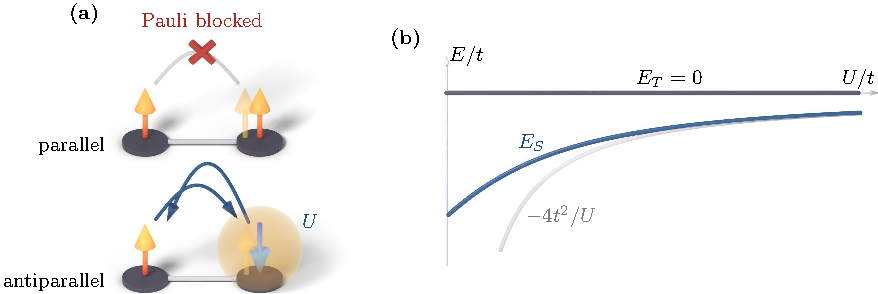
\includegraphics{figures/pdf/s06f02_dimer.pdf}
\end{aqmfigure}
